\chapter{Analyzing Muon Properties} \label{sec:analysis}

Providing the ability to perform studies on the systematic uncertainties of muon cross-sections is one of the main goals and advantages of the simulation library PROPOSAL.
The main questions for improved cross-sections in simulations are, what effects do these improvements have on simulated events and their agreement with measured data.
Thereby, the effects can either be analyzed in simulated event distributions regarding only the particle physics properties independent of the detector.
In air shower simulations, the longitudinal and lateral distribution of the occurring particle types are that kind of relevant parameters, that can be compared.
Regarding muons in deep underground experiments, the energy and zenith distribution of the incoming muon flux as well as the energy loss behavior are the most important parameters.% depending on an accurate description of the survival probability or propagated range.
% Since the atmospheric muon flux at the earth's surface is not completely understood, which was already described as \textit{muon puzzle} in \secref{sec:muon_puzzle}, both, the generation processes and the propagation processes needs

The effects can also be analyzed after the full simulation chain including detector-specific thresholds or resolutions of the reconstruction.
After the question, if the effect is still visible on the detector level, the step is to find out how much it can affect further analysis and if it needs to be taken into account in the calculation of systematic uncertainties.
If this is the case, one can finally try to measure these effects.

In this chapter, these three approaches of detector independent and detector specific simulation studies as well as an outlook on potential measurements of the muon cross-sections are discussed, focusing on large volume neutrino detectors.

%

\section{Propagation Effects of Improved Muon Cross Sections}

For muon energies above a TeV, the energy loss is dominated by pair production for small energy losses and bremsstrahlung for large energy losses.
Both interactions contribute nearly equally to the average energy loss as shown in \figref{fig:dedx_all}.
Next to the widely used standard cross-sections, which for both interactions the parametrizations were calculated by the group labeled \textit{KelnerKokoulinPetrukhin} (KKP95), also improved bremsstrahlung and pair production cross-sections labeled \textit{SandrockSoedingreksoRhode} (SSR19) are implemented in PROPOSAL.
The differences between these parametrizations are an improved treatment of the screening effect for both processes and radiative corrections for bremsstrahlung, which is described in \secref{sec:interactions}.
As shown in \figref{fig:dedx_kkp_ssr}, the average energy loss of the bremsstrahlung increases by around \SI{2}{\%}, mainly driven by the additional radiative corrections.
The improved screening for pair production decreases the average energy loss by half a percent.
\begin{figure}
    \centering
    \begin{subfigure}[t]{0.47\textwidth}
        \centering
        \includegraphics[width=\textwidth]{./plots/results_icrc/dedx_compare_brems.pdf}
        \caption{Average energy loss of bremsstrahlung.}
        \label{fig:dedx_brems_kkp_ssr}
    \end{subfigure}
    \hfill
    \begin{subfigure}[t]{0.47\textwidth}
        \centering
        \includegraphics[width=\textwidth]{./plots/results_icrc/dedx_compare_epair.pdf}
        \caption{Average energy loss of pair production.}
        \label{fig:dedx_epair_kkp_ssr}
    \end{subfigure}
    \caption{The average energy loss of muons in ice comparing the \textit{KelnerKokoulinPetrukhin} (KKP95) parametrization and the \textit{SandrockSoedingreksoRhode} (SSR19) parametrization.}
    \label{fig:dedx_kkp_ssr}
\end{figure}

The overall increase of the average energy loss further affects the survival probability and the distribution of incoming muons for underground detectors.
This slightly changes the range distribution to smaller propagated lengths as shown in \figref{fig:range_ssr_kkp}.
The expected change in the energy distribution at a certain distance towards smaller muon energies due to the increased loss is also observed, shown in \figref{fig:energy_ssr_kkp}.
However, the number of muons losing just a small amount of their energy is increased, which can be explained due to the higher stochasticity.
But these are rather small effects compared to the introduced error of an energy loss cut, shown in \figref{fig:cont_rand_mu}.
\begin{figure}
    \centering
    \begin{subfigure}{0.47\textwidth}
        \centering
        \includegraphics[width=\textwidth]{./plots/results_icrc/plot_range_dist.pdf}
        \caption{The range distribution of \num{e6} muons propagated until they decay.}
        \label{fig:range_ssr_kkp}
    \end{subfigure}
    \hfill
    \begin{subfigure}{0.47\textwidth}
        \centering
        \includegraphics[width=\textwidth]{./plots/results_icrc/plot_energy_dist.pdf}
        \caption{The muon energy distribution of \num{e7} muons after propagating \SI{1}{km}.}
        \label{fig:energy_ssr_kkp}
    \end{subfigure}
    \caption{Comparison of propagating muons through ice with an initial energy of \SI{10}{TeV} and an energy loss cut of \SI{500}{MeV}. The propagation with the default cross-sections for bremsstrahlung, i.e. the \textit{KelnerKokoulinPetrukhin} (KKP95) parametrization, is compared with the \textit{SandrockSoedingreksoRhode} (SSR19) parametrization.}
    \label{fig:range_energy_ssr_kkp}
\end{figure}

For large volume detectors like neutrino telescopes, also the energy loss behavior inside the detector is relevant, especially for the energy reconstruction or event selection.
Thereby, the combined effect of increased bremsstrahlung and decreased pair production cross-section is even more significant and can directly be seen, as shown in \figref{fig:sec_dist_ssr_kkp}.
\begin{figure}
    \centering
    \begin{subfigure}{0.47\textwidth}
        \centering
        \includegraphics[width=\textwidth]{./plots/results_icrc/plot_sec_dist.pdf}
        \caption{Comparing the bremsstrahlung and pair production parametrization of \textit{KelnerKokoulinPetrukhin} (KKP95) with the \textit{SandrockSoedingreksoRhode} (SSR19) parametrization.}
        \label{fig:sec_dist_ssr_kkp}
    \end{subfigure}
    \hfill
    \begin{subfigure}{0.47\textwidth}
        \centering
        \includegraphics[width=\textwidth]{./plots/results_icrc/plot_sec_dist_mu.pdf}
        \caption{Comparing the effect of including the muon pair production, where the muons are further propagated taking into account also their energy losses.}
        \label{fig:sec_dist_mupair}
    \end{subfigure}
    \caption{Comparison of the secondary energy distribution of \num{e7} muons propagated with an initial energy of \SI{10}{TeV} through \SI{100}{m} of ice with an energy loss cut of \SI{500}{MeV}.}
    \label{fig:sec_dist_compare}
\end{figure}
Also, the effect of including the muon pair production is compared, shown in \figref{fig:sec_dist_mupair}, slightly indicating more low energy losses driven by the additional low energy muons.
But this is less significant compared to the clear deviation due to the bremsstrahlung and pair production cross-sections.
The next step is now to analyze if this deviation is still visible on detector level, described in the next section.
The results of this section were also presented in \cite{Soedingrekso19ICRC}.
% The main task of this study is to find out which detector resolution and event statistic is required to measure the effect of a higher bremsstrahlung cross section of a few percent regarding the differences in the energy loss spectrum.

%

\section{Feasibility study to measure the Bremsstrahlung Cross Section} \label{sec:study}

The significant effects of the improved muon cross-section on the energy loss distribution in \figref{fig:sec_dist_compare} raise the question of how much this affects the energy reconstruction for neutrino telescopes which rely on an accurate description of the continuous and stochastic losses.
This would then also affect e.g. the energy flux measurements of astrophysical neutrinos.
A further question is, whether the energy loss distribution can even be measured.
This would validate the theory of both pair production and bremsstrahlung calculations, which dominate in different parts of the energy loss spectrum.

There have been measurements of the muon cross-section with the ATLAS detector below \SI{100}{GeV} \cite{Amaral01MuonMeasure} and less precise measurements using cosmic-ray induced muons up to \SI{1}{TeV} \cite{Sakumoto92TeVMuonMeasure}, where the ionization is still dominating the energy loss.
Since the stochastic processes start to dominate at energies around a TeV, such a measurement is still required.
Hereby, large volume neutrino telescopes like IceCube, measuring muons with energies from below a TeV up to the PeV region, provide the unique opportunity to perform such a measurement, which would be the first in this energy region.

In this section, a feasibility study is described to measure the cross-section using the energy loss profile along the produced tracks inside a cubic kilometer scale detector.
Regarding the reconstruction of single energy losses along the muon track, small energy losses can not be distinguished and rather measured as continuous loss, especially for a sparsely instrumented detector, like neutrino telescopes, while large stochastic losses can be identified and reconstructed as a single high energy loss or cascade.
Since bremsstrahlung interactions are dominating those high energy losses, this study focuses on measuring the bremsstrahlung cross-section.

Also, the efficiency of the photomultipliers and the spectral index of the muon flux are included as further systematic parameters to analyze their correlation with this study.
Although both systematic parameters will have larger impacts on the energy loss distribution, this will affect the whole secondary distribution, while bremsstrahlung only affects the largest losses.

The created toy Monte-Carlo simulation and reconstruction is adapted to imitate the simulation and reconstruction methods used in the IceCube experiment.
Also, the statistic of the used event sample and energy spectrum are based on public IceCube analysis.
However, they can be applied to any neutrino telescope configuration.
A generic framework is created, where the configuration of the detector scale or the reconstruction performance can be adjusted to perform the study for another dedicated detector.
% The overall procedure is to histogram all muons with the same energy when entering the detector.
% % The chosen muon energy bins and energy loss bins are described in table \ref{}.
% Then, the energy loss histograms for each muon energy bin are stacked together.
% The resulting energy loss histogram for each muon energy bin are produced for different multipliers scaling the bremsstrahlung cross section, detector efficiencies and spectral indices of the flux.
% The differences between these histograms are interpolated.
% These interpolations are used to fit the three parameters of a given histogram.
% Finally the performance of the fit is estimated for three different resolution settings.

One has to point out that the scope of this study is not to fine-tune the analysis on the simulation model or a specific detector configuration and produce as many simulations to extract the best achievable results out of this toy Monte-Carlo.
This is a feasibility study if a measurement of the Bremsstrahlung is possible for neutrino telescopes and tries to be as simple and resource efficient as it can.

This study was developed in collaboration with Mirco Hünnefeld, Maximilian Meier, and Alexander Sandrock and the results were presented in \cite{Soedingrekso20ICPPA}.

%

\subsection{Event Sample}

For the dataset of this study, a single muon sample with a decent statistic of muon energies above a TeV and a good measurement of the energy loss profile is required.
This is currently only achievable using cubic kilometer sized neutrino telescopes.
Although atmospheric muons are abundant for neutrino telescopes, they are of limited use regarding a measurement with the energy loss distribution.
Most cosmic-ray induced muons arrive as low energy stopping muons, which are not in the relevant energy region, or they arrive in bundles, where the separation of single muons and the reconstruction of their energy losses is not feasible.
Therefore, neutrino-induced muons are used in this analysis, since they don't arrive as bundles and they are in the relevant energy region.

Neutrino-induced muons are produced with a hadronic cascade at the neutrino vertex, containing on average $\sfrac13$ of the neutrino energy (see \figref{fig:nu_xsection_y}), which cannot be distinguished from an energy loss.
This disturbs especially the large stochastic losses, which are the focus of this study.
However, most of the muons are produced outside of the detector propagating inside without any detectable light of the vertex.
This can for example be indicated by the difference of two orders of magnitude in the number of neutrino events between a track sample \cite{IceCube2016Aachen} and cascade sample \cite{IceCube20Cascades}.
Therefore this effect can be neglected for this study.
Trident processes, here the muon pair production, can also create a bundle out of a single muon.
But these muons are usually comparably low energetic and do not propagate large distances or change the energy loss profile significantly, shown in \figref{fig:sec_dist_mupair}.
\begin{figure}
    \centering
    \includegraphics[width=0.8\textwidth]{./plots/results_study/plot_event_spectrum.pdf}
    \caption{Event spectrum of selecting up-going muon events using ten years of IceCube data. \cite{Stettner19ICRC}. A power law is fitted for events with a reconstructed muon energy between \SI{1}{TeV} and \SI{100}{TeV}.}
    \label{fig:study_event_spectrum}
\end{figure}

A comparable dataset is the sample of up-going, thereby neutrino-induced, muon tracks measured in ten years by the IceCube Collaboration \cite{Stettner19ICRC}, further described in \cite{IceCube2016Aachen}.
As shown in \figref{fig:study_event_spectrum}, the event distribution of the neutrino sample consists of roughly \num{245000} events between \SI{1}{TeV} and \SI{100}{TeV} and approximately follows a power-law spectrum with a spectral index of \num{1.6}.
This is a relatively flat spectrum compared to the steeper spectral index of the atmospheric or astrophysical flux, which are approximately \num{3.7} and \num{2.3} respectively.
However, this can be explained with the detector acceptance and the higher probability of higher energetic muons to get detected and included in the dataset \cite{IceCube2016Aachen}.
% The energy in \figref{fig:study_event_spectrum} is reconstructed using the average energy method, described in \secref{sec:IceCube}, also called \textit{truncated energy}.
% The resulting muon spectrum will be sightly steeper due to energy losses of the muons while propagating to the detector.

%

\subsection{The Toy Monte-Carlo}

The simulation uses the PROPOSAL library for the Monte-Carlo propagation of the muons.
The default cross-section for ionization, $e^+e^-$ pair production, bremsstrahlung, and inelastic nuclear interaction are used including the LPM effect, while the bremsstrahlung can be scaled according to a given multiplier.
To save computation time, all further corrections are turned off, i.e. the $\mu$ pair production and the weak interaction, scattering and deflection calculations as well as exact time calculations.
The medium is set to ice and an energy loss cut of \SI{500}{MeV} between stochastic and continuous losses is used, which is also used in the IceCube simulation chain.

The initial energy of the propagated muons is sampled from a power-law $\propto E^{-\gamma}$ with a spectral index of $\gamma=1$ in the energy range between \SI{100}{GeV} and \SI{1}{PeV}.
With this flat spectrum also high energy muons get simulated with a decent statistic to estimate their contribution to this study.
The transformation to a more realistic energy spectrum of the muons can be considered by re-weighting the events.

The maximum distance muons are allowed to propagate is varied between \SI{100}{m} and \SI{1}{km} and is randomly chosen from a uniform distribution to take into account the different propagation lengths inside the detector.
Although a description of the length distribution for the used muon sample is not publicly available, a uniform distribution is a conservative assumption, since the selection of muons favors long tracks.
Especially as the propagation lengths inside the detector can also reach \SI{1.5}{km}.

A smearing of the energy loss profile, compared to the differential cross section is included intrinsically in the simulation setup as just the starting muon energy (that is the energy when the muon enters the detector) for all the energy losses of the track is used and not the muon energy at each energy loss.
However, on average, a TeV muon is not losing much of its energy within a kilometer, as shown in \figref{fig:energy_ssr_kkp}.
Regarding initial energies around \SI{10}{TeV} and a propagated distance of \SI{100}{m}, energy losses of more than \SI{10}{\%} of the muon energy occur less than once per muon, which can be seen in \figref{fig:sec_dist_ssr_kkp}.
Since this study is focused on high energy losses, this does not affect the analysis significantly. 
Besides, this effect is included in all energy loss distributions and here, just the differences between these distributions are of interest.

% Due to the limited resolution of neutrino telescopes, since not every single energy loss can be reconstructed, the energy losses are combined together along a track in e.g. \SI{15}{m} track segments.
% This further smears the energy loss distribution decreasing the amount of measured small energy losses.
% In addition to the stochastic energy losses, the continuous losses are added to the energy losses per segment according to their length in the segments.

For real simulation of the detector, further processes and acceptance corrections are considered in the simulation chain, like noise, triggers, and the generation and propagation of Cherenkov photons.
Out of the measured time series of the pulses by the photodetectors, further reconstruction methods are applied to parametrize.
These simulations are specific for each detector and most often produced by closed source software.
Furthermore, these steps are computationally expensive compared to the fast muon simulation.
To create a toy Monte Carlo including semi-realistic detector effects, the following smearing and cutoff steps are performed to extract the measured energy losses of a muon.
\begin{enumerate}
    \item The position or vertex of each stochastic loss is smeared out. Thereby, the energy loss is not deposited at a single point, but along the track according to a Gaussian distribution with the width $\sigma_V$.
    \item Each muon track is divided into equidistant track segments of a certain length $\Delta X$.
    \item The expected energy loss in each segment is accumulated from the smeared out stochastic losses distributed on the track segments and the number of continuous losses according to their fraction in each segment.
    \item To model hits in the photo multipliers of the detector, the expected energy losses per track segment in MeV are sampled using a Poisson distribution.
    \item Due to the finite energy resolution, these hits, representing the energy, are further smeared out using a Gaussian distribution. The width of the Gaussian distribution $\sigma_E = \sigma_{\text{base}} \cdot f_E$ consists of a scaling parameter $f_E$ and an energy-dependent resolution $\sigma_{\text{base}}$ similar to the energy resolution of IceCube \cite{IceCube2014Ereco} shown in \figref{fig:study_energy_resolution_curve}.
    \item The energy measured in each track segment can be scaled according to a given efficiency of the photomultipliers, taking into account a further systematic uncertainty parameter.
    \item Finally, a threshold $E_{\text{cut}}$ is applied and segments with an energy below this threshold are discarded, taking into account the limited detector sensitivity.
\end{enumerate}
Independent of the simulation of the measured energy loss of the segments, the measured length the muons are propagated inside the detector is simulated by smearing out the true length using a Gaussian distribution with the width $\sigma_L$.
\begin{figure}
    \centering
    \includegraphics[width=0.8\textwidth]{./plots/results_study/energy_resolution_curve.pdf}
    \caption{The energy-dependency of the resolution of the energy reconstruction $\sigma_E$ for the three resolution settings listed in \tabref{tab:study_resolutions}. The shape of the curve is taken from \cite{IceCube2014Ereco}.}
    \label{fig:study_energy_resolution_curve}
\end{figure}
\begin{table}
    \centering
    \caption{For this study, three different sets of resolution settings
        were chosen: low, medium, and high resolution.}
    \label{tab:study_resolutions}
    \begin{tabular}{l | c c c}
        \toprule
        Resolution Parameter & High & Medium & Low \\
        \midrule
        Vertex resolution $\sigma_V$ / m & 2 & 5 & 10 \\
        Track segment length $\Delta X$ / m & 5 & 15 & 30 \\
        Energy resolution factor $f_E$ & 0.5 & 1.0 & 1.5 \\
        Energy cutoff $E_{\mathrm{cut}}$ / MeV & 10 & 50 & 100 \\
        Length resolution $\sigma_L$ / m & 10 & 50 & 100 \\
        \midrule
        Energy Uncertainty Cut & 0.2 & 0.4 & 0.6 \\
        Coefficient of Determination $R^2$ & 0.9 & 0.95 & 0.995 \\
        \bottomrule
    \end{tabular}
\end{table}

This study is performed using three different settings for the detector resolution, listed in \tabref{tab:study_resolutions}; one considered as baseline setting, one with a low resolution, and one with high resolution.
These three settings are comparable to the main IceCube array, the DeepCore, and the IceCube-Gen2 expansions respectively.
For an example muon track, \figref{fig:study_ereco_eloss_profile} shows the energy loss profile reconstructed with the three resolution settings compared to the true energy loss profile.
\begin{figure}
    \centering
    \includegraphics[width=0.8\textwidth]{./plots/results_study/ereco/energy_loss_reco_v1_00000014.png}
    \caption{The final energy loss profile for an example muon track reconstructed with the three resolution settings according to \tabref{tab:study_resolutions}. The true energy losses use a track segment length of \SI{2}{m} to compare the results.}
    \label{fig:study_ereco_eloss_profile}
\end{figure}

%

\subsection{Energy Reconstruction} \label{sec:study_ereco}

Next to the two \enquote{measured} parameters, the length and the energy losses, also the reconstructed energy is required for this study, which is estimated using the energy losses per track segment.
The energy of the muon when it enters the detector is reconstructed using two independent reconstruction methods to validate their results.

To calibrate both energy reconstruction methods a dataset with \num{e6} muons and a spectral index of $\gamma=1$ is created.
A larger energy range from \SI{1}{GeV} to \SI{100}{PeV} is used to avoid boundary effects and also correctly reconstruct the edge cases.
To use just events with enough information, only events with a track length $l > \SI{100}{m}$ are selected for the calibration.

In the so-called \enquote{truncated energy} method the linear behavior of the overall continuous energy loss to the muon energy (c.f. \figref{fig:dedx_all}) is used.
It is similar to the method described in \cite{IceCube2014Ereco}, which is the default energy reconstruction for high energy muons in IceCube.
This dependency is mainly driven by the pair production interaction, where the amount of low energy losses just increases linearly with the muon energy.
On the other side, the bremsstrahlung-driven energy losses are equally distributed in the log space of the muon energy.
This results in mainly stochastic losses that are uncorrelated with the muon energy.
Therefore the stochastic losses are cut out for this method and the \enquote{truncated} energy loss segments are used.
Here, the \SI{10}{\%} of the track segments with the highest losses are ignored.
The dependency of the remaining energy losses and the muon energy is calibrated using a spline-fit.
For the baseline resolution, the calibration and the performance of this method are shown in \figref{fig:study_ereco_trunc}.
For the other two resolutions, this is shown in \secref{sec:study_ereco_calib}
\begin{figure}
    \centering
    \begin{subfigure}{0.47\textwidth}
        \centering
        \includegraphics[width=\textwidth]{./plots/results_study/ereco/te_model_e0_400_b1500_000_l5000_000_v2000_000_c1000_000.pdf}
        \caption{The calibration curve, shown in red.}
        \label{fig:study_ereco_trunc_calib_base}
    \end{subfigure}
    \hfill
    \begin{subfigure}{0.47\textwidth}
        \centering
        \includegraphics[width=\textwidth]{./plots/results_study/ereco/energy_correlation_te_model_e1_000_b1500_000_l5000_000_v500_000_c50_000__fraction_1.000.pdf}
        \caption{The performance of the reconstruction.}
        \label{fig:study_ereco_trunc_perf_base_show}
    \end{subfigure}
    \caption{The truncated energy reconstruction for the baseline resolution setting. On the left side, the correlation between the average energy loss of the truncated track segments and the true muon energy is calibrated, using a spline fit. On the right side, the performance using this calibration is evaluated on an independent dataset.}
    \label{fig:study_ereco_trunc}
\end{figure}

Below a TeV, the Ionization is dominating the muon energy loss and there is no correlation between the continuous energy loss and the muon energy due to the nearly flat dependency (c.f. section \figref{fig:dedx_all}).
This limits the resolution at lower energies for this method and in general.
Another approach at these energies is the track length, but even at several \SI{100}{GeV} the average propagated distance of muons in ice exceeds a kilometer.
As this analysis is more focused on muons above a TeV, more advanced methods improving the truncated energy reconstruction are not considered here.

Varying the cross-sections and changing the relation between small continuous losses and large stochastic losses might affect the energy reconstruction.
However, the analysis should be sensitive to changes in the energy loss distribution, while other parameters should remain stable.
A shift also in the energy reconstruction would mean, that muons of different energy regions would get compared, directly lead to a different energy loss profile, disturbing the cross-section measurement.

Therefore, a second and independent method to reconstruct the energy using a neural network is implemented, also as a cross-check to the truncated energy method.
This machine learning method has shown comparable or even improved performances in IceCube compared to the best likelihood-based energy proxies like truncated energy \cite{Huennefeld17ICRC, Huennefeld19VLVNT}.
In principle, the network can learn the same truncated energy method described above, while using the available information to learn also the other reconstruction methods, e.g. the track length correlation or using the stochastic losses as a lower limit.
Here, a combination of convolutional layers, to learn the correlation between the neighboring segments, and dense layers, combining the elements, is used to estimate the energy.
The rather small network architecture for this light-weighted study is listed in \tabref{tab:nn_layers_ereco}.
\begin{table}
    \caption{The convolutional neural network architecture used for the energy reconstruction.}
    \label{tab:nn_layers_ereco}
    \centering
    \begin{tabular}{l | c c c c}
        \toprule
         & \multicolumn{4}{c}{Details} \\
        Layer Name & Kernel size & Filters & Activation & Units \\
        \midrule
        Batch Normalization & \multicolumn{4}{l}{Normalization of reconstructed energy loss input} \\ \cline{2-5}
        Convolution 1D & 7 & 15 & relu & \\
        Convolution 1D & 7 & 15 & relu & \\
        Max Pooling 1D & 2 & & & \\
        Convolution 1D & 7 & 15 & relu & \\
        Convolution 1D & 7 & 15 & relu & \\
        Max Pooling 1D & 2 & & & \\
        Convolution 1D & 7 & 15 & relu & \\
        Convolution 1D & 7 & 5  & relu & \\  \cline{2-5}
        Flatten & \multicolumn{4}{l}{Flatten layer} \\  \cline{2-5}
        Dense & & & relu & 32 \\
        Dense & & & relu & 16 \\
        Dense & & & None & 1\\
        \bottomrule                          
    \end{tabular}
\end{table}

Comparing the performance of these two energy reconstruction methods, regarding Figure \ref{fig:study_ereco_trunc_perf_base_show} and \ref{fig:study_ereco_nn_base_perform_all_show}, the truncated energy method performs slightly better at the relevant energies above a TeV.
The neural network provides stable performances also at lower energies, probably using the track length dependency for these events.
But in general, both methods provide similar results, shown in detail in \secref{sec:study_ereco_perform_all}, and can be used as realistic energy reconstruction methods.
\begin{figure}
    \centering
    \begin{subfigure}{0.47\textwidth}
        \centering
        \includegraphics[width=\textwidth]{./plots/results_study/ereco/energy_correlation_nn_model_e1_000_b1500_000_l5000_000_v500_000_c50_000__fraction_1.000}
        \caption{All events.}
        \label{fig:study_ereco_nn_base_perform_all_show}
    \end{subfigure}
    \hfill
    \begin{subfigure}{0.47\textwidth}
        \centering
        \includegraphics[width=\textwidth]{./plots/results_study/ereco/energy_correlation_nn_model_e1_000_b1500_000_l5000_000_v500_000_c50_000__fraction_0.500.pdf}
        \caption{\SI{50}{\%} of the events.}
        \label{fig:study_ereco_nn_base_perform_0.5_show}
    \end{subfigure}
    \caption{The performance of the neural network reconstruction of the muon energy for the baseline resolution. On the right side, an uncertainty cut is applied filtering \SI{50}{\%} of the best reconstructed events compared to the full event sample on the left side.}
    \label{fig:study_ereco_nn_base_perform}
\end{figure}
% \begin{table}[]
%     \caption{The performance of the truncated energy reconstruction method is shown for the three resolution settings. All performance values are calculated in log-space. MSE is the mean squared error, MAE the mean absolute error, and the resolution is computed according to \cite{Ereco}.}
%     \label{tab:te_energy_reco}
%     \centering
%     \begin{tabular}{l | ccc | ccc}
%         \toprule
%          & \multicolumn{3}{c}{Truncated Energy} & \multicolumn{3}{c}{Neural Network} \\
%         Name & High & Medium & Low & High & Medium & Low \\
%         \midrule
%         Res. Mean & $-0.062$ & $-0.065$ & $-0.111$ & 0.005 & $-0.062$ & $-0.090$ \\
%         Res. Std. & 0.292 & 0.480 & 0.775 & 0.349 & 0.426 & 0.503 \\
%         Pearson & 0.984 & 0.956 & 0.895 & 0.978 & 0.964 & 0.949 \\
%         Spearman & 0.988 & 0.977 & 0.923 & 0.980 & 0.967 & 0.950 \\
%         MSE & 0.089 & 0.235 & 0.613 & 0.122 & 0.185 & 0.261 \\
%         MAE & 0.203 & 0.305 & 0.538 & 0.248 & 0.293 & 0.360 \\
%         Resolution} & 0.341 & 0.429 & 0.713 & 0.401 & 0.468 & 0.560 \\
%         \bottomrule                          
%     \end{tabular}
% \end{table}

To discard the muons with large mis-reconstructed energies, disturbing the energy loss spectrum and reducing the sensitivity of this study, an estimation of the uncertainty of the energy reconstruction is required.
Recent developments show, that such uncertainty estimators provide accurate and robust estimations of the real deviation, useful in IceCube analysis \cite{Huennefeld17ICRC}.
Again a neural network is used with nearly the same network architecture as for the energy reconstruction but using the absolute function for the activation.
The network then returns the absolute value of the estimated deviation of the reconstructed energy in the log space.
The increase in the performance of the energy reconstruction using a cut of the energy uncertainty estimator is indicated in \figref{fig:study_ereco_nn_base_perform_0.5_show}.
However, this uncertainty cut reduces also the size of the data sample and for each resolution setting a trade-off between a high sample statistic and good reconstructed events is made for the selection.

For a final check of the energy reconstruction, its correlation to the scaling of the bremsstrahlung cross-section has to be analyzed.
As already mentioned, a correlation between these parameters would be a circle conclusion, since the energy loss distributions are created according to the reconstructed energy.
If this also changes, the effect of a changing energy loss profile is a circle.
Therefore, both parameters have to be uncorrelated, at least inside the parameter space this study is focused on.
In principle, the energy reconstruction of course depends also on the bremsstrahlung cross-section as described above.
A higher bremsstrahlung cross-section results in more high energy losses and fewer lower energetic losses.
This changes the ratio between small continuous losses and high stochastic losses the reconstruction methods are tuned on.
But the energy reconstruction should be robust against small changes in the bremsstrahlung cross-section, as the same amount of stochastic losses should get truncated.
\begin{figure}
    \centering
    \includegraphics[width=\textwidth]{./plots/results_study/reco_test/TruncatedEnergyResolution.pdf}
    \caption{The pull distribution of reconstructed energies using the truncated energy method for the three resolution settings and muon energies. The multiplier, scaling the bremsstrahlung cross-section is varied between \num{0.9} and \num{1.1}, and the mean and standard deviation for each multiplier dataset is estimated.}
    \label{fig:study_ereco_pull_te}
\end{figure}

Regarding changes of $\pm \SI{10}{\percent}$ in the bremsstrahlung cross-section, no changes of the energy reconstruction are observed, as shown in \figref{fig:study_ereco_pull_te}.
Just for large scalings of the bremsstrahlung by orders of magnitudes, the relation between continuous and stochastic losses changes significantly and the correlation gets visible, shown in \figref{fig:study_ereco_pull_te_extreme}.
This independence of the energy reconstruction from small bremsstrahlung changes is observed for each resolution setting and both reconstruction approaches (see \secref{sec:study_pull_dist}).
In general, the cross-check of the energy reconstruction was successful, since both approaches produce similar and robust results.

%

\subsection{Parameterizing the Energy Loss Distribution}

% With the measured length and energy losses and with the reconstructed muon energy and its uncertainty the energy loss distributions can be created.
Before creating the energy loss distributions, an event selection consisting of two pre-cuts is performed discarding mis-reconstructed events.
First, only events propagating at least \SI{100}{m} through the detector are selected to avoid corner clippers and make sure, that a sufficient part of the track is visible to reconstruct the relevant information.
The second cut is performed on the energy uncertainty parameter and can be adapted for each resolution setting.
For this study, the energy loss cut for the three resolution settings is listed in \tabref{tab:study_resolutions}.

Furthermore, only muon energies between \SI{1}{TeV} and \SI{100}{TeV} are selected, since lower energetic muons are dominated by ionization losses and higher energies are lacking of statistics.
The selected muon range is divided into three equally sized bins in $\log_{10}$-space between \SI{1}{TeV} and \SI{10}{TeV} and two bins also equally distributed in $\log_{10}$-space between \SI{10}{TeV} and \SI{100}{TeV}.
This corresponds approximately to the energy ranges listed in \tabref{tab:study_energy_ranges}.
\begin{table}
    \caption{Energy ranges of reconstructed muon energies selected for this study.}
    \label{tab:study_energy_ranges}
    \centering
    \begin{tabular}{c | S[table-format=3.2] S[table-format=3.2]}
        \toprule
        \multicolumn{2}{c}{Energy Range / TeV}  \\
        {Lower Bound} & {Upper Bound} \\
        \midrule
        1 & 2.15 \\
        2.15 & 4.64 \\
        4.64 & 10 \\
        10 & 31.6 \\
        31.6 & 100 \\
        \bottomrule
    \end{tabular}
\end{table}

Using the reconstructed energy losses per track segment, an energy loss histogram is created for each muon energy bin according to the weight of the given energy spectrum.
% Hence, the Monte Carlo simulation is created with a small spectral index of 1 to have enough statistic also at higher energies, the events or their energy loss distribution needs to be weighted to the assumed spectral index.
Assuming a Poisson distribution for the content of each energy loss bin, the normalized energy loss distribution $H$ and its error $E$ can be expressed by
\begin{align}
    H = \frac{\sum L_i w_i}{\sum w_i d_i}
    \qquad \text{and} \qquad
    E = \frac{\sum L_i w_i^2}{\sum w_i d_i}.
\end{align}
with the energy loss histograms $L$ the energy weight $w$ and the propagated distances $d$ per event $i$.
Since the energy losses histogram is just comparable with the same propagated distance, they are normalized by the weighted propagation length.
Using the produced energy loss distributions, the main task is to parameterize and fit the differences between these energy loss histograms according to the fit parameters.
The variations of the three fit parameters are listed in \tabref{tab:study_interpol_set}.
\begin{table}
    \caption{Interpolation settings for the three fit parameters.}
    \label{tab:study_interpol_set}
    \centering
    \begin{tabular}{l ccc}
        \toprule
        Fit Parameter & Bremsstrahlung & DOM Efficiency & Spectral Index \\
        \midrule
        Interpolation Points & 9 & 9 & 9 \\
        Interpolation Range & [0.9, 1.1] & [0.9, 1.1] & [1.5, 1.9] \\
        Fit Range & [0.95, 1.05] & [0.95, 1.05] & [1.6, 1.8] \\
        Baseline Value & 1.0 & 1.0 & 1.7 \\
        Order of Interpolation & cubic & quadratic & quadratic \\
        \bottomrule
    \end{tabular}
\end{table}

For each scaling of the bremsstrahlung cross-section (Multiplier) \num{1e7} muons are simulated between \SI{100}{GeV} and \SI{1}{PeV} with a spectral index of \num{1}.
Then, each bremsstrahlung multiplier dataset is reconstructed with the different efficiency of the photomultipliers (DOM efficiency).
Therefore the different DOM efficiency data points are correlated and not created using independent Monte-Carlo simulations.
However, this approximation was made to reduce the runtime of the simulation.
This gets even more relevant for the spectral index (Gamma) as these datasets are just re-weighting the events for each bremsstrahlung simulation and DOM efficiency reconstruction data set.
The interpolation points are placed with an equidistant spacing between each other and span a grid of $9\times9\times9$ points in the fit parameter space for each bin, shown in \figref{fig:study_interpol_3d_show}.
\begin{figure}
    \centering
    \includegraphics[scale=0.45, angle=270]{./plots/results_study/create_m/e0.500_b500.000_l1000.000_v200.000_c10.000/normmethod_2_energyreco_1/Multiplier/interpol/interpol_param_muon_energy_bin_3.pdf}
    \caption{One dimensional interpolation of the differences between the energy loss histograms created with different bremsstrahlung multiplier. The baseline resolution is used and reconstructed muon energies between \SI{10}{TeV} and \SI{31.6}{TeV} using neural networks are selected. A coefficient of determination threshold of \num{0.9} is used to mark all energy loss bins (red colored legend box), which would not be included in a fit of the bremsstrahlung.}
    \label{fig:study_1d_interpol_mu3_te}
\end{figure}

% This is one reason why the Bremsstrahlung data points fluctuate the most.

To get an impression of how the energy loss bins change by varying the fit parameter and how the shape looks, one-dimensional interpolations are created.
Thereby only one parameter is changed, while for the other two parameters, the default value is used.
For the Bremsstrahlung multiplier, this is shown in \figref{fig:study_1d_interpol_mu3_te}, and in \secref{sec:study_append_interpol} for the other settings.
Compared to the DOM efficiency and spectral index, the effect of the bremsstrahlung multiplier is less significant.
One reason is, that the bremsstrahlung datasets are independent of each other, while the other two interpolations are built on the same dataset.
But the main reason for this is, that the Bremsstrahlung is just a smaller effect compared to the DOM efficiency and the spectral index, which are considered in every IceCube analysis.
Also without smearing of the reconstructions, using the Monte-Carlo truths of the secondary spectrum directly to create these interpolations, the bremsstrahlung data points do fluctuate significantly more compared to the other parameters where the smearing of the reconstructions are included.

The used polynomials for each fit variable are also listed in \tabref{tab:study_interpol_set}.
Thereby a trade-off is made between a small degree of freedom and a precise description while just interpolating the real physical changes and no fluctuation and do overfitting.
For the DOM efficiency and the spectral index, the slight curvature can be well expressed with a quadratic polynomial.
A cubic polynomial is used for the bremsstrahlung multiplier as it allows to describe more structures while still limiting overfitting.

Energy loss bins, which do not significantly change or have a slope, or where the interpolation does not describe the data points, due to large fluctuations, should not be considered for this analysis.
Therefore the coefficient of determination
\begin{align}
    R^2 = 1 - \frac{\sum (y - f(x))^2}{\sum (y - \bar{y})^2}
\end{align}
is calculated for each bin to be able to exclude bins with a bad interpolation or no significant changes.
Thereby, $y$ represents the difference between the energy loss bins and $f(x)$ the interpolation function.
\begin{figure}
    \centering
    \begin{subfigure}{0.47\textwidth}
        \centering
        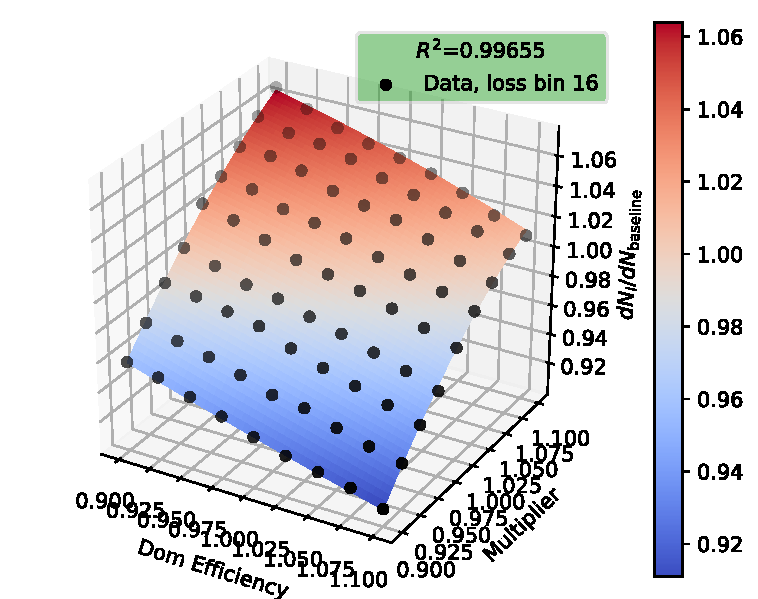
\includegraphics[width=\textwidth]{./plots/results_study/interpol_energy_bin_3_2d.pdf}
        \caption{2D-Interpolation of the DOM efficiency and the bremsstrahlung multiplier.}
        \label{fig:study_interpol_2d_show}
    \end{subfigure}
    \hfill
    \begin{subfigure}{0.47\textwidth}
        \centering
        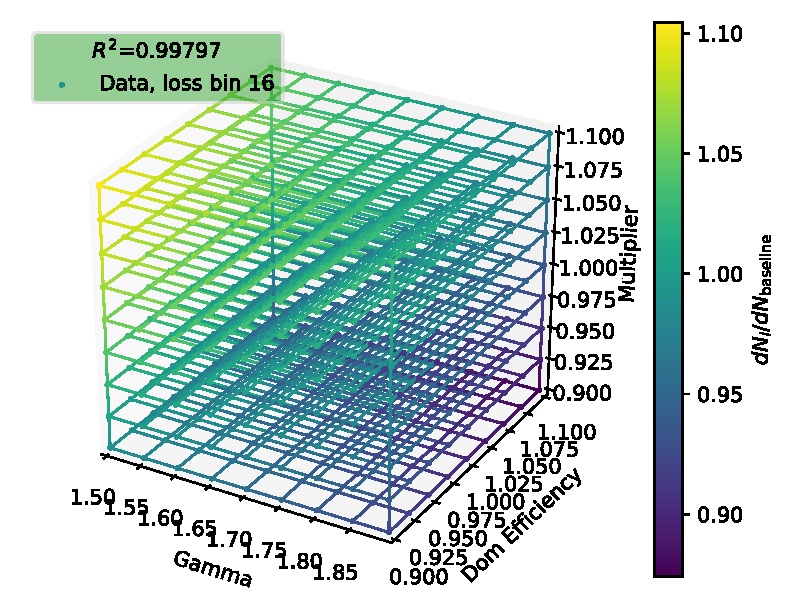
\includegraphics[width=\textwidth]{./plots/results_study/interpol_energy_bin_3_3d.pdf}
        \caption{3D-Interpolation of the spectral index, DOM efficiency, and the bremsstrahlung multiplier.}
        \label{fig:study_interpol_3d_show}
    \end{subfigure}
    \caption{The interpolation of the differences of the energy loss histogram for muons with reconstructed energies between \SI{1}{TeV} and \SI{31.6}{TeV} using neural networks for the energy reconstruction. The high resolution setting is considered, here. For the 2D-interpolation the color bar equals the z-axis, and is shown for a clearer understanding. In the 3D-interpolation only the color bar represents the bin difference.
    The coefficient of determination $R$ is calculated.}
    \label{fig:study_interpol_show}
\end{figure}

Due to the correlations between the fit variables, one-dimensional interpolations do not take into account all these effects.
This can be seen in \figref{fig:study_interpol_2d_show} in a 2D interpolation of the bremsstrahlung multiplier and the DOM efficiency.
Although it is also possible to treat the spectral index rather independently of the other two processes in a 1D interpolation, assuming negligible correlation to the other parameters.
In this analysis, a 3D-interpolation, shown in \figref{fig:study_interpol_3d_show}, is used with the function
\begin{align}
    f(x_{\text{brems}}, x_{\text{eff}}, x_{\text{gamma}}) 
        &= a_0
        + a_1 x_{\text{brems}} + a_2 x_{\text{brems}}^2 + a_3 x_{\text{brems}}^3 \nonumber \\
        &+ a_4 x_{\text{gamma}} + a_6 x_{\text{gamma}}^2
        + a_6 x_{\text{eff}} + a_7 x_{\text{eff}}^2 \\
        &+ a_8 x_{\text{brems}} \cdot x_{\text{gamma}}
        + a_9 x_{\text{brems}} \cdot x_{\text{eff}}
        + a_{10} x_{\text{gamma}} \cdot x_{\text{eff}} .\nonumber
\end{align}
The threshold for the coefficient of determination $R^2$ can be set for each resolution setting.
For this study, the values are already listed in \tabref{tab:study_resolutions}.

%

\subsection{Performance of the Measurement}

With these interpolations, a Poisson Likelihood is defined to describe the bin contents of the energy loss distributions.
A Marcov-Chain-Monte-Carlo (MCMC) sampling is then applied to estimate the three parameters including their correlations, shown exemplarily in \figref{fig:study_mcmc_show}.
\begin{figure}
    \centering
    \includegraphics[width=0.8\textwidth]{./plots/results_study/test_m/e1.000_b1500.000_l5000.000_v500.000_c50.000/normmethod_2_energyreco_0/corner_plots/corner_domeff0.953_gamma1.674_brems1.04_mubin01234.pdf}
    \caption{Sampling result of the MCMC estimation. The blue lines represent the true values.}
    \label{fig:study_mcmc_show}
\end{figure}
% The settings for the MCMC are listed in table \ref{}.

To estimate the performance of the bremsstrahlung multiplier measurement for the different resolutions, Monte-Carlo simulation sets, each with random bremsstrahlung multipliers and fixed systematic parameters are produced propagating \num{e6} muons.
The results for the baseline resolution setting are shown in \figref{fig:study_result_corr}.
Further results with different resolution settings or energy reconstruction methods are shown in \secref{sec:study_perform_result_all}.
The values outside the fit range, defined in \tabref{tab:study_interpol_set}, are on the one site calculated to analyze the effect.
But on the other side, these values are discarded from the performance estimation, due to boundaries effects biasing parameters at the edge of the ranges towards the center.

There is no notable difference in the performance between the truncated energy and the neural network approach to estimate the muon energy.
For the high resolution, the bremsstrahlung multiplier can be estimated within $\pm\SI{1}{\%}$ and for the baseline resolution, this increases to $\pm\SI{4}{\%}$ (shown in \figref{fig:study_result_pull}).
For the low resolution, it is not feasible to estimate the bremsstrahlung multiplier, since the likelihood landscape for the \SI{68}{\%} central interval already exceeds the boundaries of the interpolated range (shown in \tabref{tab:study_interpol_set}).
However, boundary effects can also be observed for higher resolutions, like in \figref{fig:study_mcmc_show}.

The DOM efficiency can be measured with the highest precision and the spectral index with still high accuracy.
The precision and the bremsstrahlung multiplier with the lowest accuracy, which is expected as the effect of the Bremsstrahlung on the energy loss distribution is already smaller and just significant at higher energy losses.
\begin{figure}
    \centering
    \includegraphics[width=\textwidth]{./plots/results_study/test_m/e1.000_b1500.000_l5000.000_v500.000_c50.000/normmethod_2_energyreco_1/performance/show_all2.pdf}
    \caption{Correlation of the true values and the estimated results of the MCMC samplings with the baseline resolution settings for the spectral index, the DOM efficiency and the bremsstrahlung multiplier. The muon energy is reconstructed using the neural network. The region below 0.95 and above 1.05 is neglected for the performance to avoid boundary effects during the MCMC sampling at the edge of the allowed interpolation region. The error represents the \SI{68}{\%} central interval and the best fit value, the median.}
    \label{fig:study_result_corr}
\end{figure}

\begin{figure}
    \centering
    \includegraphics[width=\textwidth]{./plots/results_study/test_m/e1.000_b1500.000_l5000.000_v500.000_c50.000/normmethod_2_energyreco_1/performance/show_all.pdf}
    \caption{Pull distribution of the estimated results of the MCMC samplings with the baseline resolution settings for the spectral index, the DOM efficiency and the bremsstrahlung multiplier. The muon energy is reconstructed using the neural network. The region below 0.95 and above 1.05 is neglected for the performance to avoid boundary effects during the MCMC sampling at the edge of the allowed interpolation region. The error represents the \SI{68}{\%} central interval and the best fit value, the median.}
    \label{fig:study_result_pull}
\end{figure}

Concluding the results, it is possible to measure the bremsstrahlung multiplier with high resolutions similar to a cubic kilometer-sized DeepCore detector, in the percent level.
Regarding resolution setting similar to IceCube, a measurement is still feasible, but with higher uncertainties of around \SI{4}{\%}.
For a detector as sparsely instrumented as the IceCube-Gen2 detector or with similar resolutions, a measurement of the bremsstrahlung using the same techniques is not feasible.
Thereby the amount of events surviving the cuts of a track length and in particular of the uncertainty of the energy estimation is reduced significantly with nearly no muons left to analyze.
However, since Gen2 is designed to detect more muons at higher energies, the setup should be adapted to these energies and sizes.

The spectral index and the DOM efficiency can be measured in every setup, also for low resolutions.
In this analysis, the spectral index is only taken into account as a nuisance parameter, as it describes only the spectrum of muons entering the detector, not relevant for other analyses.
The DOM efficiency, however, is a systematic parameter relevant for every analysis.
A measurement or reduction of the region, that needs to be considered for the DOM efficiency would directly increase the sensitivity for these analyses.
But a more precise measurement of the DOM efficiency can be performed using a stopping muon sample with their minimal Ionizing muons.
Further possible measurements of muon properties or systematics are described in the next section.

%

\section{Outlook of Measurements using Atmospheric Muons} \label{sec:global_muon_fit}

The study described above using a neutrino-induced muon sample is one way to measure muon properties using large volume detectors like IceCube.
To measure further parts of the muon cross-section, other approaches including atmospheric muon samples are required.
The big benefit in using atmospheric muons is the increased sample size of several orders of magnitude, being able to make a more rigorous selection demanding a high reconstruction quality.

A dataset selecting stopping muons mainly consists of single muons \cite{Hoinka17Master, Ninfa19Master}.
Usually, the last surviving muon is the highest energetic particle of the muon bundle produced in the air shower.
Most of these muons are far below a TeV and with no stochastic loss and therefore not interesting for the study described in the previous section.
However, at these energies, the ionization is dominating the energy loss with its nearly energy independent and constant energy loss probability.
Either the DOM efficiency or the ionization cross-section can be measured while fixing the other parameter.% or while estimating this parameter also in another cross-section analysis.

Next to the calibration advantages, this sample can also be used to measure the muon energy distribution at the surface.
The range of these muons to the surface can be determined using their reconstructed direction for zenith angles below \SI{80}{\degree}, where the incoming muon flux is dominated by atmospheric muons and the neutrinos contribution is sub-dominant.
Then, the energy distribution of the muons can be unfolded using the relation between the range and average energy loss, described in \secref{sec:dedx}.
Furthermore, the differences between the muons traveling short distances through the ice and muons traveling long distances can be used to verify the muon cross-sections assuming both originate from the same distribution.
Due to the relative comparison of the same sample, most systematic parameters cancel out.

Another approach is by using a leading muon sample selecting atmospheric muon bundles where a single muon contains most of the bundle energy.
For bundles with an equal energy distribution between the muons, the event signature is a homogeneous bright track where all the stochastic losses by the different muon are 'washed' out.
If a single muon contains most of the bundle energy, there is a higher fluctuation of the brightness along the track and more visible stochasticity.
With this sample also higher energetic muons can be selected, but couldn't be used for the analysis above as it depends on the relation of high stochastic and low continuous energy losses.
Fitting the Bremsstrahlung cross-section with this sample would therefore be a circle conclusion as just events with higher energy losses are selected.
Due to the higher energy range, this dataset is used in an ongoing analysis to estimate the prompt atmospheric muon spectrum, similar to \cite{Fuchs16PhD, Fuchs16ECRS}.

A goal would finally be to combine these three datasets low energetic stopping muons, muons and neutrino-induced single muons, and high energetic leading muons.
Due to shared systematic parameters, a precise measurements of muon properties can be performed.
Although large volume neutrino telescopes are not designed to measure muon properties, they provide the unique opportunity to analyze and verify muon physics at energies not feasible for accelerator detectors of the current and the next generation.
